\subsection{Referencia de conectores}
A continuación presentamos una referencia a los conectores utilizados en los diagramas que se presentaran en las siguientes secciones. Los conectores \emph{no-standard} utlizados son especificados mas abajo.

\begin{figure}[H]
	\centering
	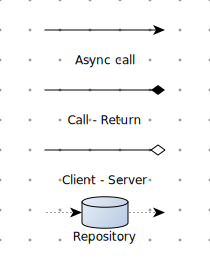
\includegraphics[scale=0.6]{graficos/call_reference.png}
	\caption{Referencia de conectores.}
\end{figure}

\subsubsection{Conectores no estandar}

\begin{itemize}
		%Completar con conectores no standard!
		%Agregar asi:
		\NonStandardConector{A non standard conector name}{A non standard conector description.}
\end{itemize}

\subsection{Subsistema de Query}

En el siguiente diagrama presenta el \textsf{Subsistema de Query} donde dada una consulta por productos (\textbf{query}) se arma la respuesta al usuario que realizó la consulta. En este diagrama se encuentran ejemplificados los \emph{casos de uso} 7, 8, 9, 10, 11 y 12.

\begin{figure}[H]
	\centering
	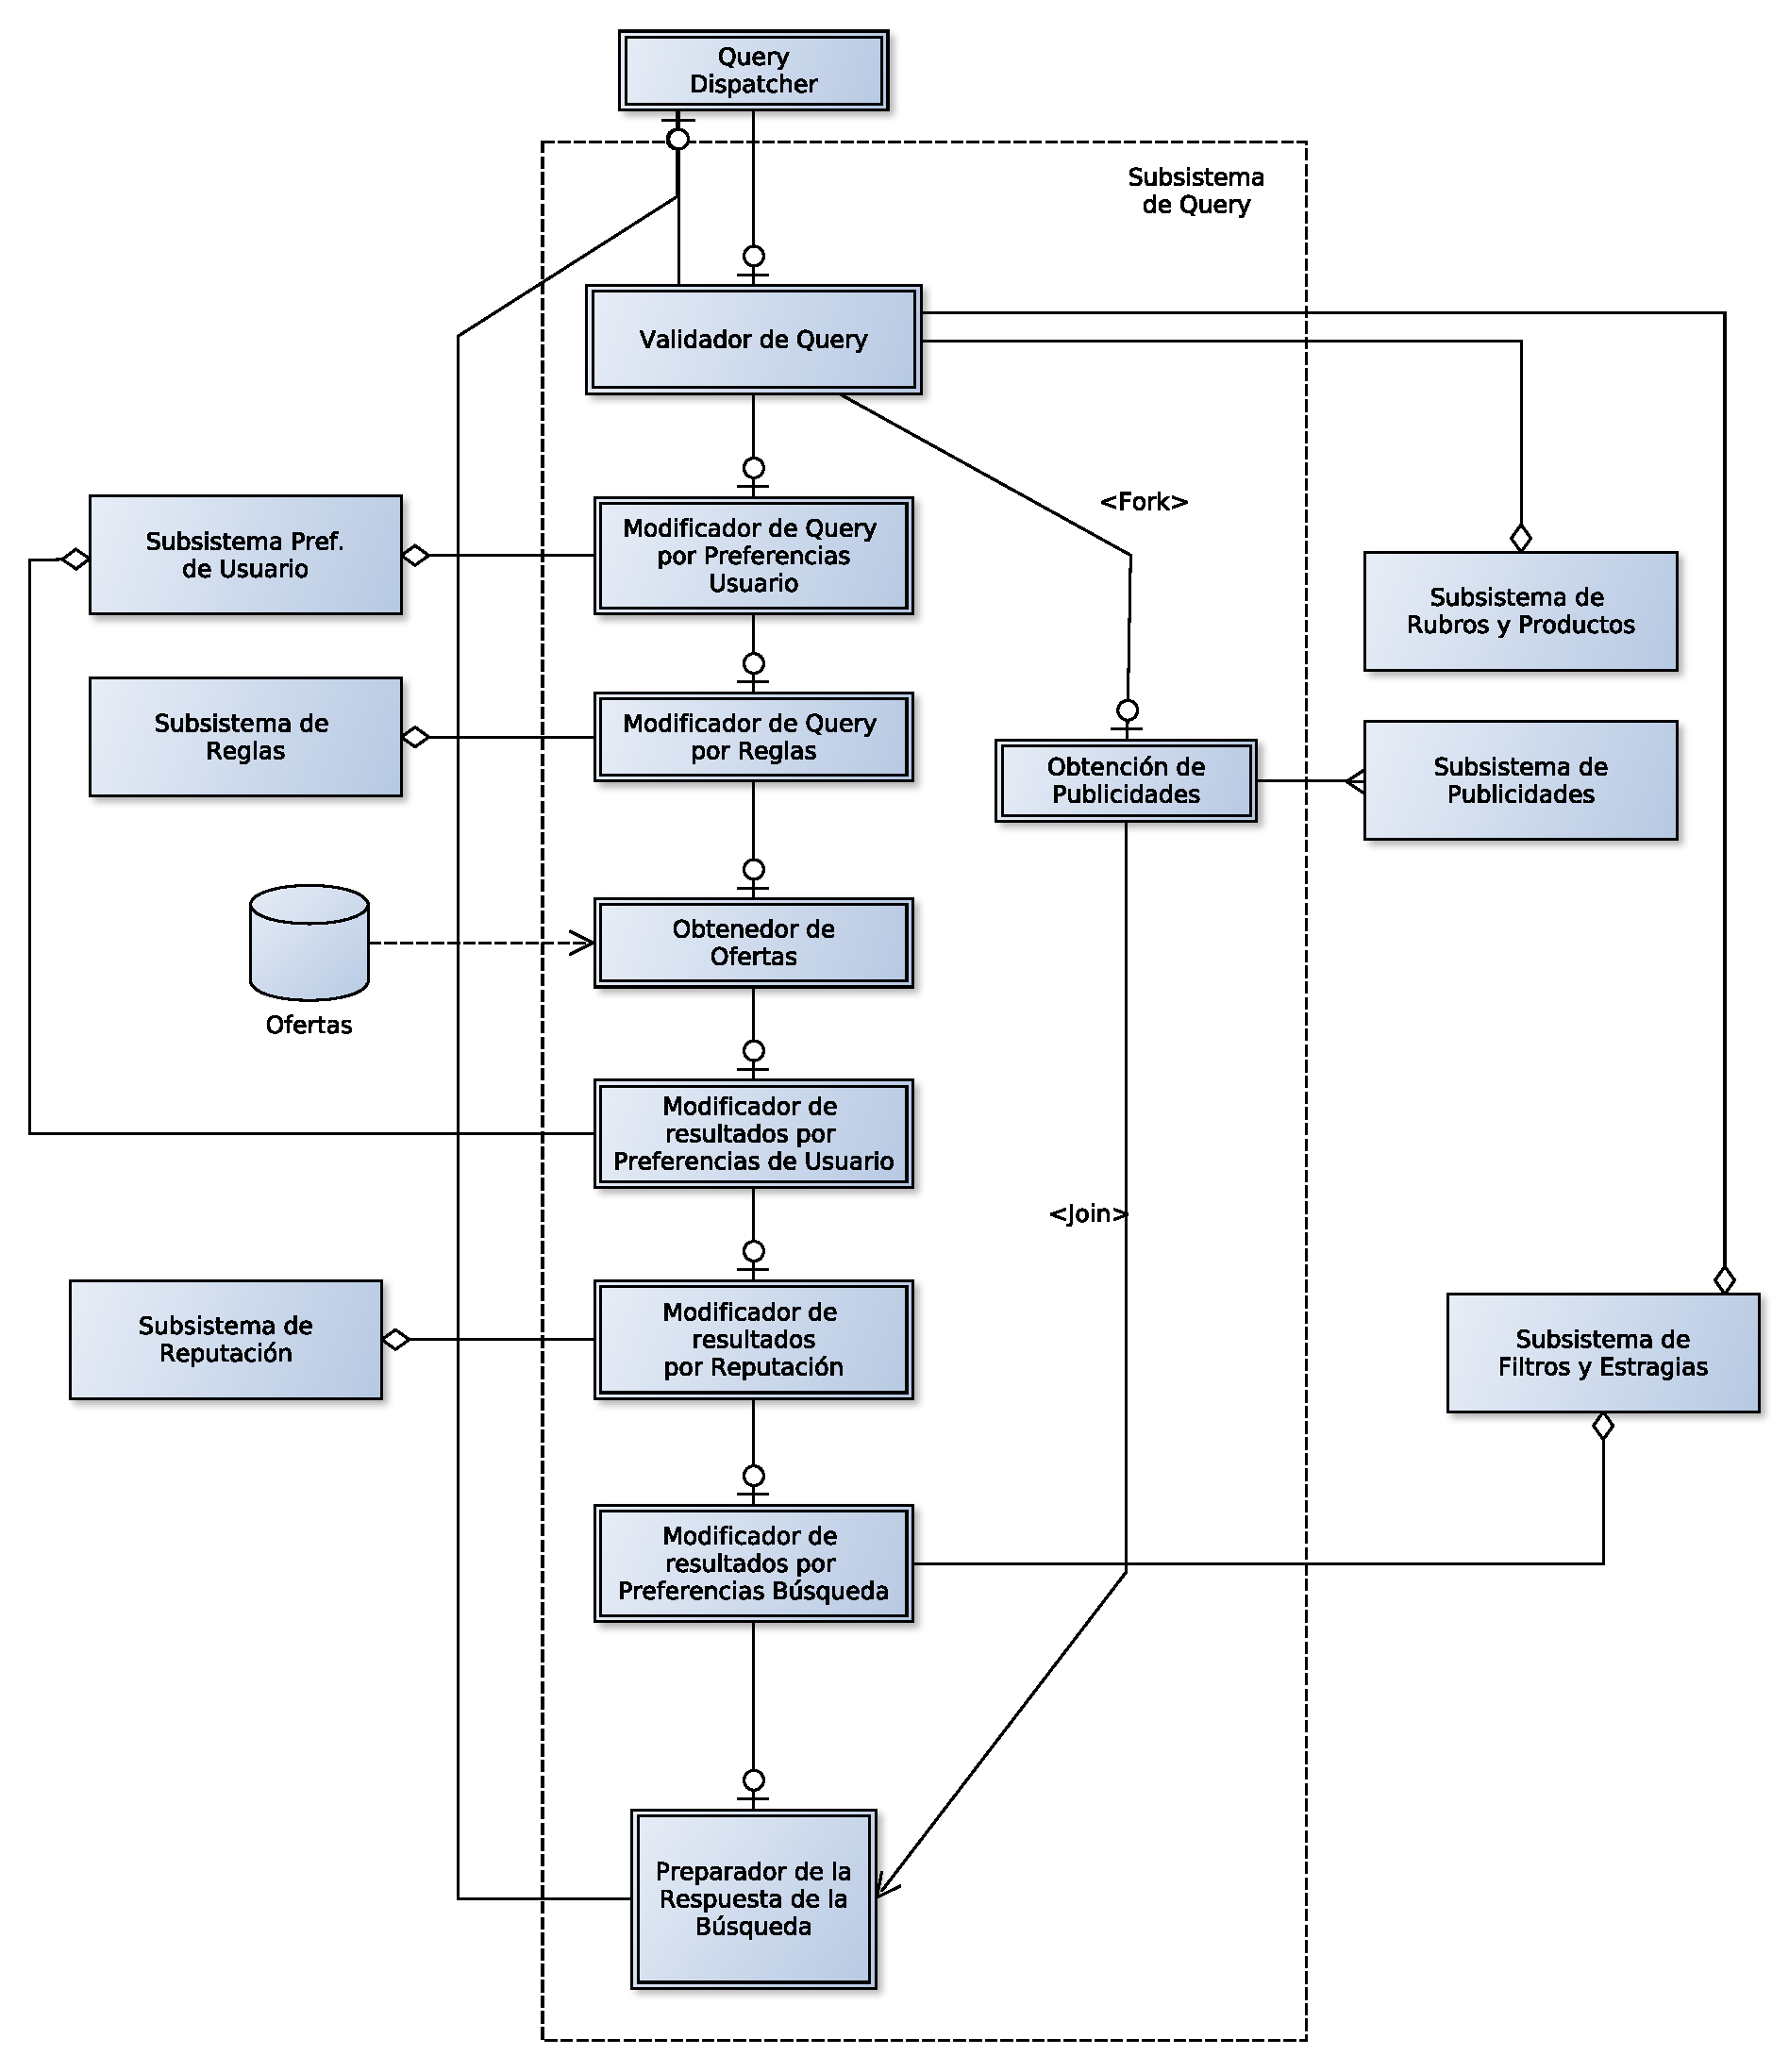
\includegraphics[width=\textwidth]{graficos/arch/subsistema_query.png}
	\caption{Diagrama arquitectónico con el detalle del \textsf{Subsistema de Query}.}
\end{figure}

\subsection{Interfaz movil}

\begin{figure}[H]
	\centering
	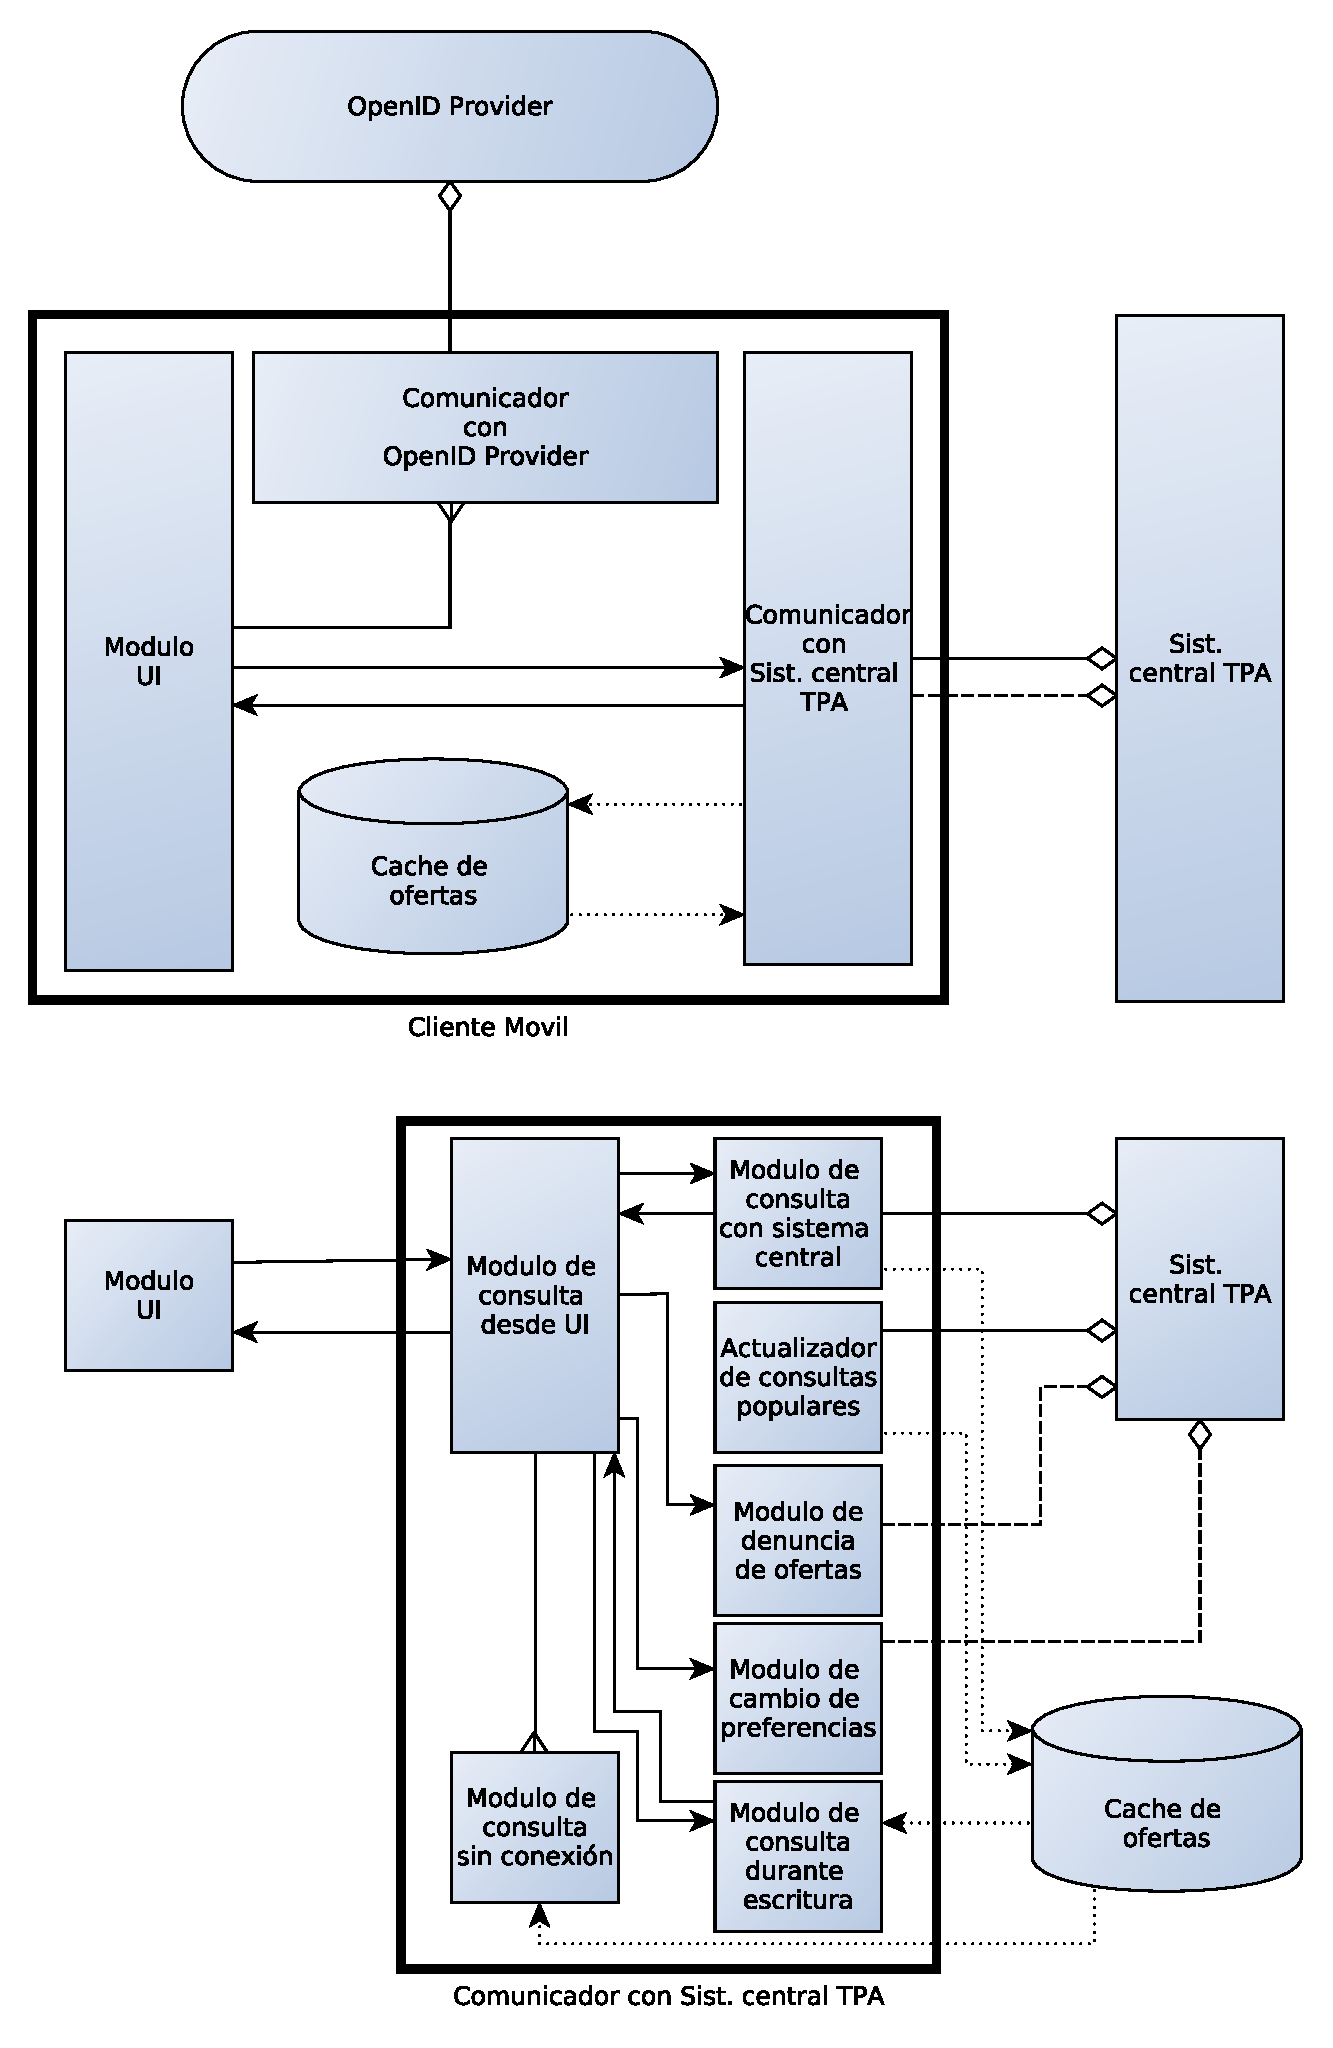
\includegraphics[width=\textwidth]{graficos/arch/Cliente_movil.png}
	\caption{Diagrama arquitectónico con el detalle del \textsf{Cliente movil}.}
\end{figure}

\subsection{Interfaz web}

\begin{figure}[H]
	\centering
	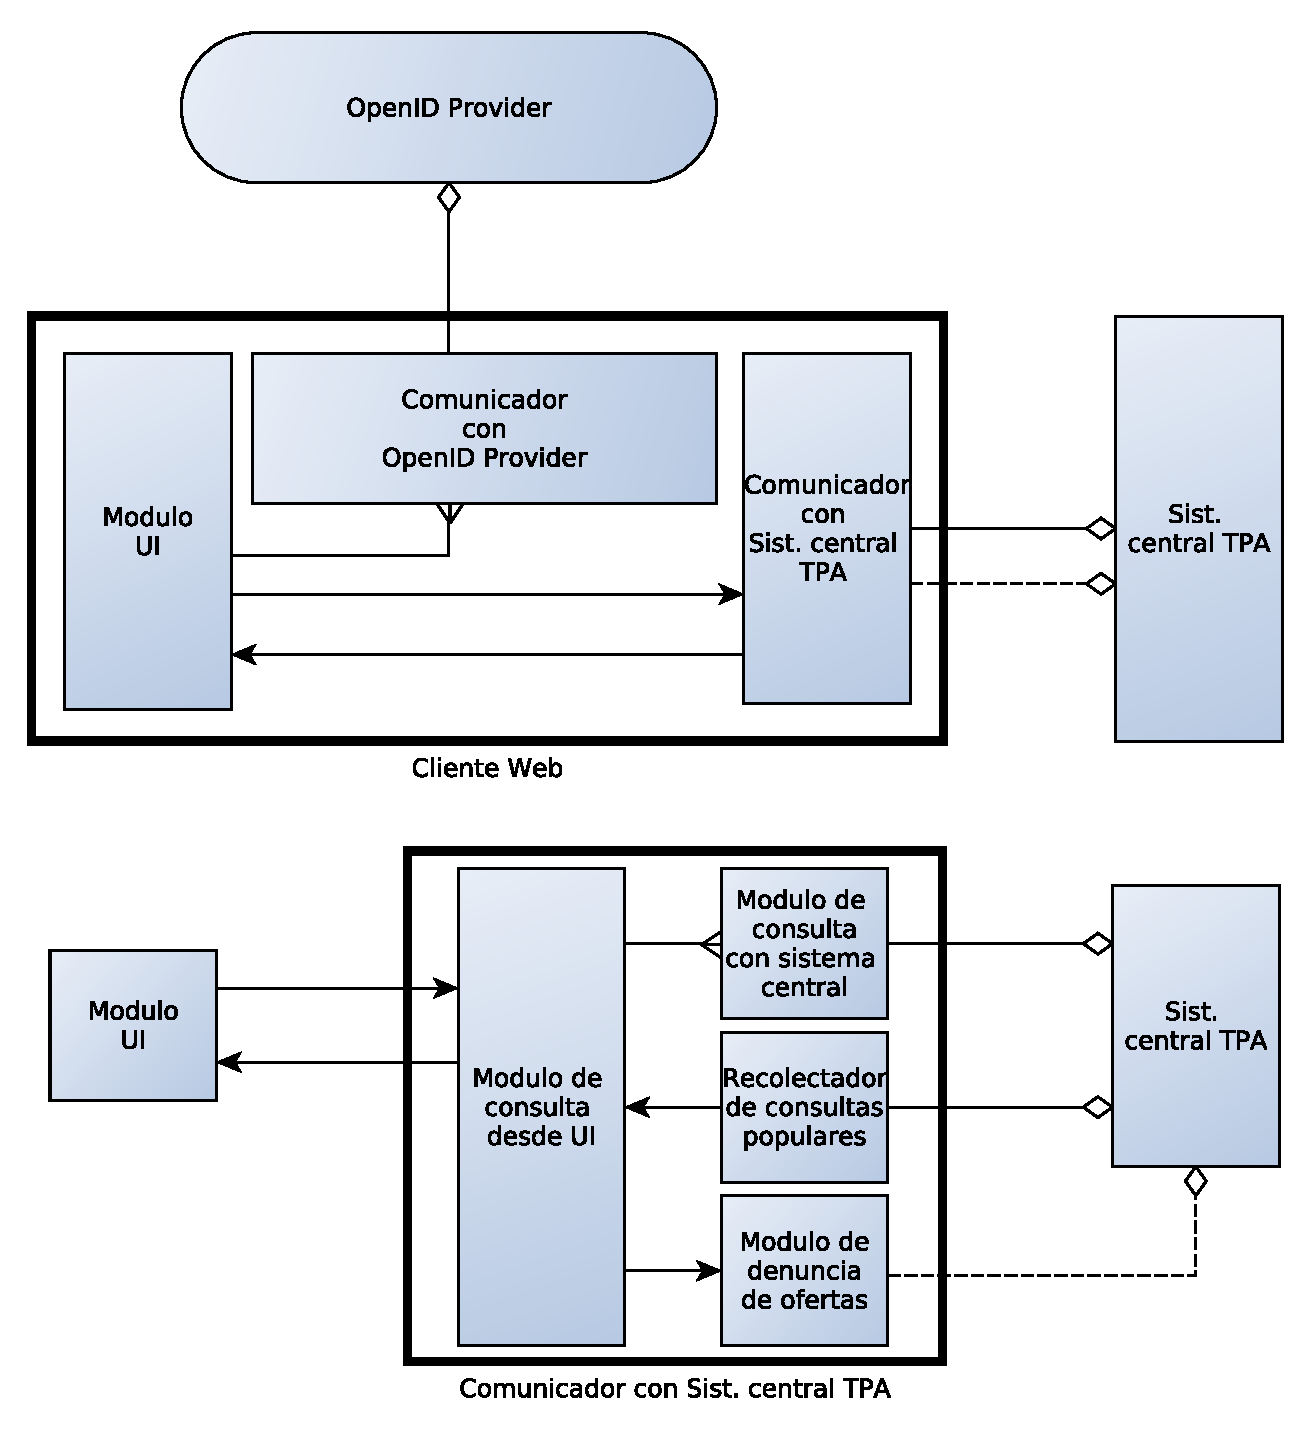
\includegraphics[width=\textwidth]{graficos/arch/Cliente_web.png}
	\caption{Diagrama arquitectónico con el detalle del \textsf{Cliente web}.}
\end{figure}


\subsection{Sistema de Detección de Spam}
Nota: hay que aclarar el significado de spam... leer anteultimo parrafo del tp
\begin{figure}[H]
	\centering
	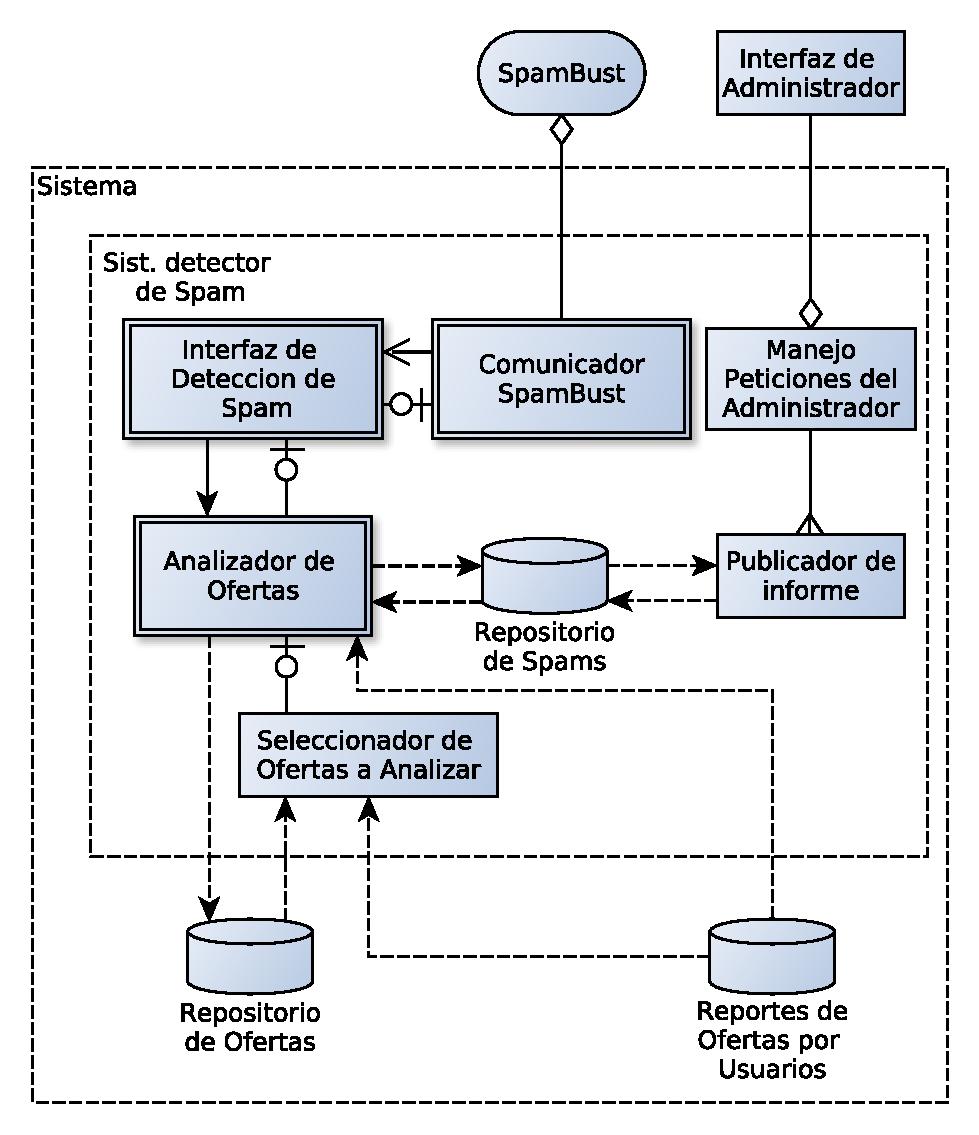
\includegraphics[width=\textwidth]{graficos/arch/Sistema_deteccion_spam.png}
	\caption{Diagrama arquitectónico con el detalle del \textsf{Sistema de Detección de Spam}.}
\end{figure}

\subsection{Sistema de Obtención de Datos}
Nota: la mescla entre nombre de ingle y espa~nol es cualquiera...
nota2: que eso eso de cliente servidor asincronico??
nota3: los robot hay que expandirlos, como?
\begin{figure}[H]
	\centering
	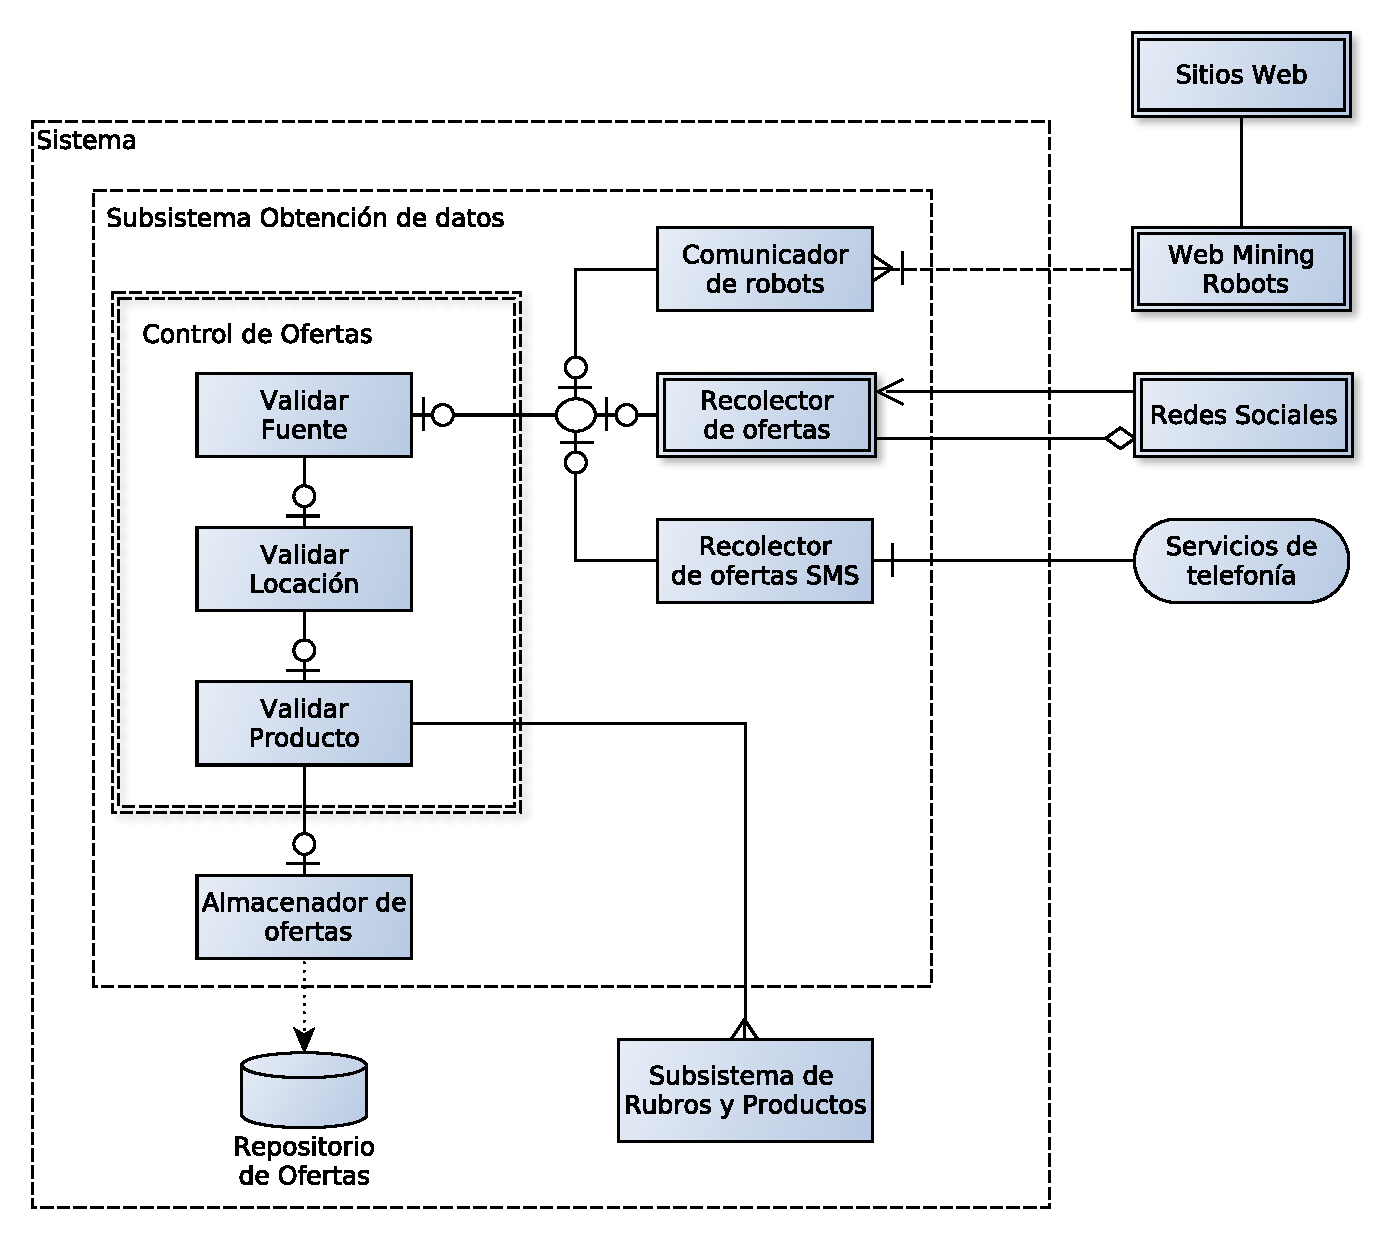
\includegraphics[width=\textwidth]{graficos/arch/Sistema_obtenedor_datos.png}
	\caption{Diagrama arquitectónico con el detalle del \textsf{Sistema de Obtención de Datos}.}
\end{figure}

